%%% File encoding is ISO-8859-1 (also known as Latin-1)
%%% You can use special characters just like ä,ü and ñ

\chapter{Main Part}

\Blindtext[1][1]

\begin{figure}[htb]
\centering
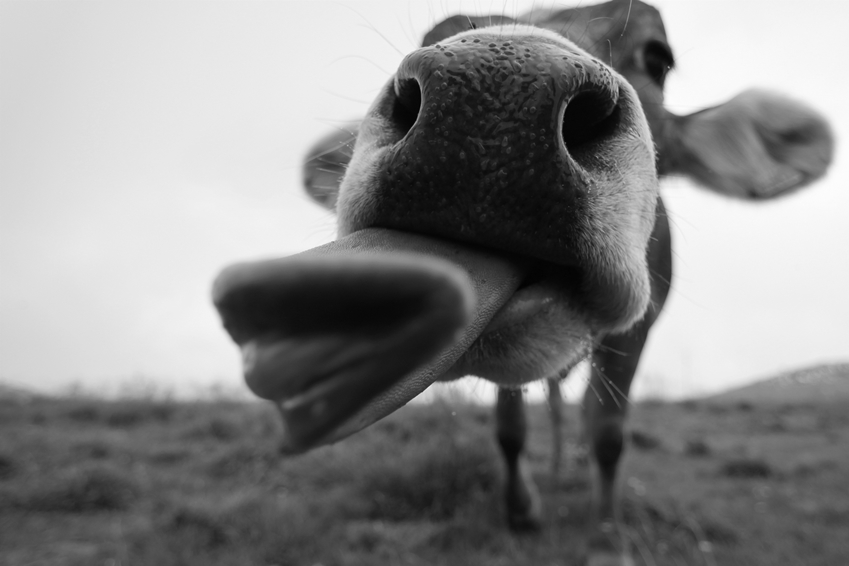
\includegraphics[width=0.9\textwidth]{03_GraphicFiles/CowLickingNose.jpg}
\captionsource{A cow licking its nose. Usage with permission of the photographer \textsc{Nicole Barth}}{Obtenido de \url{www.flickr.com/photos/46311827@N07/14885545396}, (2017)}
\label{fig:CowLickingNose}
\end{figure}

En la \figurename~\ref{fig:CowLickingNose}\myMarginnote{Reference to a figure} you see a cow that is licking its nose. The picture was taken by Nicole Barth on 11.08.2014 using a Canon EOS 500D. The original file has a resolution of $4247 \times 2831$ pixels\footnote{hola como te va}.


\begin{figure}[htb]
\centering
\begin{tikzpicture}
\begin{axis}[
axis lines = middle,
enlargelimits = true,
xlabel = {$x$},
ylabel = {$y$},
trig format plots = rad,
width = 0.9\textwidth,
height= 80mm,
title style={font=\bfseries,align=center,text width=0.7\textwidth},
title = {Example Diagram with a Line Break in the Title (using the \texttt{text width} option in the \texttt{title style})},
]
\addplot[myColorMainA,domain=0:9, line width=1pt, smooth]
{0.2*x^2};
\addplot[myColorMainB,domain=0:9, line width=1pt, smooth]
{5*sin(x)};
\end{axis}
\end{tikzpicture}
\captionsource{A scientific diagram using the \texttt{pgfplots} package by \textsc{Christian Feuersaenger} using the same colors which are also used for the layout}{Elaboración propia, (2017)}
\label{fig:ScientificDiagram}
\end{figure}

\Blindtext[2][2]

\begin{table}[htb]
\centering
\captiontable{A small table created with the \texttt{booktabs} package (example taken from the package documentation).}{Elaboración propia, (2017)}

\begin{tabular}{@{}llr@{}} \toprule
\multicolumn{2}{c}{Item} \\ \cmidrule(r){1-2}
Animal & Description & Price (\$)\\ \midrule
Gnat & per gram & 13.65 \\
& each & 0.01 \\
Gnu & stuffed & 92.50 \\
Emu & stuffed & 33.33 \\
Armadillo & frozen & 8.99 \\ \bottomrule
\end{tabular}

\end{table}


\Blindtext[2][1]

\section{Example Section}

\Blindtext[3][2]

\blinditemize

\section{Another Example Section}

\Blindtext[3][1]

\blindenumerate

\subsection{Example Sub-Section}

\blindmathpaper

\begin{figure}[htb]
\centering
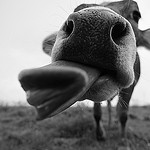
\includegraphics[]{03_GraphicFiles/CowLickingNoseSquare.jpg}
\captionsource{A cow licking its nose -- picture in square format in a native (low) resolution $150 \times 150$ pixels @ 72~dpi ($\approx 2.1$ inch). No scaling in \LaTeX{} using options in \texttt{\textbackslash includegraphics} is applied. Zoom in and see how ugly this is. See \figurename~\ref{fig:CowLickingNose} for reference.}{Elaboración propia, (2017)}
\label{fig:CowLickingNoseSquare}
\end{figure}

\subsection{Another Example Sub-Section}

\Blindtext[2][1]

\subsubsection*{Another Sub-Sub-Section}

\blindmathpaper

\paragraph{Example Paragraph}

\Blindtext[2][1]

\subparagraph{Example Sub-Paragraph}

\Blindtext[2][1]

\section{Yet Another Example Section}

\Blindtext[2][1]